\chapter{SIFT}

\section{Introduction}

\subsection{Distinctive Image Features from Scale-Invariant Keypoints}

\textbf{Goals:} \begin{itemize}
    \item Detect features in images (mainly corners)
    \item Detailed descriptor, as unique as possible
    \item Invariance in location, scale and orientation
\end{itemize}

\textbf{Applications:} \begin{itemize}
    \item Find sparse correspondences between images
    \item Estimate global rotations (stereo geometry, homographies, parametric transformations)
    \item Tracking, Structure from Motion
    \item Object detection, recognition
\end{itemize}

\subsection{The Scale-Invariant Feature Transform}

\textbf{Step 1:} Detect characteristic feature points.

\textit{Based on Gauss. scale-space using DoG; Extrema provide location and scale}

\textbf{Step 2:} Accurate localisation of key points

\textit{Subpixel refinement fitting quadratic functions; Discard points with high ration between principal curvatures}

\textbf{Step 3:} Assignment of dominant orientations

\textit{Histogram of gradients in local neighborhood; Refines orientation, fitting quadratic functions.}

\textbf{Step 4:} Computation of a suitable key point descriptor

\textit{Unit vector based on accumulated histograms of gradients; compensated by location, scale and dominant orientation}

\textbf{Remark:} Steps not difficult, lots of engineering needed for max. quality.

\section{SIFT feature detection}

\subsection{Step 1: Detection of characteristic feature points}

\subsubsection{Detection of scale-space extrema}

\textbf{Starting point: Gaussian Scale-Space of input image $f$}

Using discrete levels of smoothing again, i.e., $\sigma_0, \sigma_1, \dots$. Consecutive levels related by: $\sigma_{t+1} = k_{\sigma_t}, k > 1$. 

Scale-space is given by convolution of $f$ with increasing gaussian $f_t = G_{\sigma_t} * f$. 

\textbf{From this: DoG}

Difference of two consecutive scales: \begin{align*}
    D_t & = f_{t+1} - f_t \\
    & = G_{k\sigma_t} * f - G_{\sigma_t} * f \\
    & = (G_{k\sigma_t} - G_{\sigma_t}) * f
\end{align*}

DoG is bandpass filter, only details of a scale level survive.

\textbf{Idea:} Feature is strongest detector response in a scale, search for max. across scales for \textbf{scale invariance}.

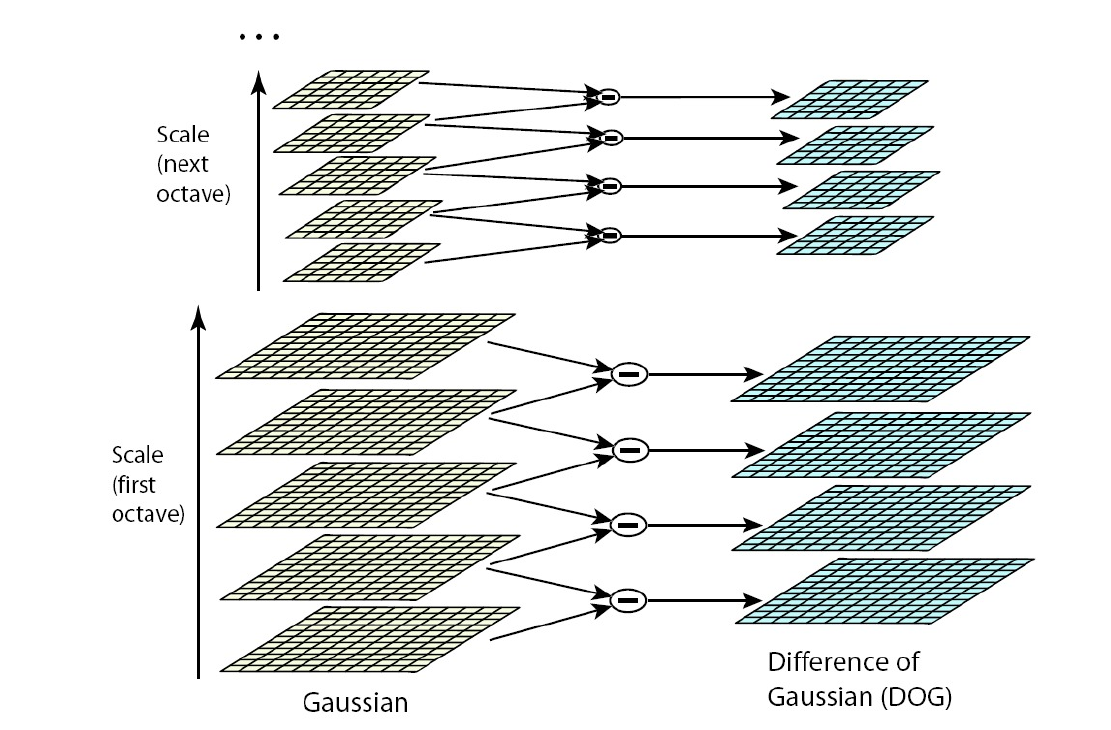
\includegraphics[width=\textwidth]{images/chap5/sift_DOG}

Here resolution is halved every octave. Original impl. uses $\sigma_0 = 0.5$ and $\rho = \sqrt{2}$.

\textbf{DoG and Laplacian-of-Gaussian}: \textit{DoG} related to scale derivative of Gaussian with following approx: $\partial_\sigma G_\sigma \approx \dfrac{G_{k\sigma} - G_\sigma}{k\sigma - \sigma}$ and the analytic derivative is the \textbf{Laplacian of Gaussian (LoG):} $$\partial_\sigma G_\sigma = \sigma \Delta G_\sigma = \sigma(\partial^2_x G_\sigma + \partial^2_y G_\sigma)$$

\textbf{Result:} DoG is approx. of scaled \textbf{LoG} with constant factor: $$G_{k\sigma} - G_\sigma \approx (k-1)\sigma^2 \Delta G_\sigma$$, but $(k-1)$ can be neglected, no influence on locations of extremal positions! $\sigma^2 \Delta G_\sigma$ is called \textbf{normalized Laplacian-of-Gaussian}! (This is also equivalence of scale space construction to heat diffusion!)

\textbf{Detection:} Filters "detect" shapes similar to their own, i.e., the LoG finds \textbf{BLOBS}. Following pictures depict scale-space for LoG:

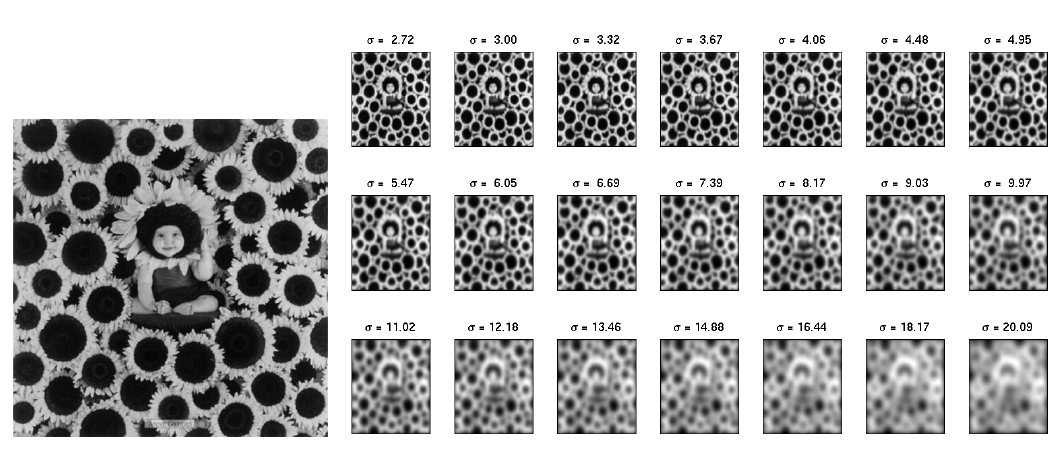
\includegraphics[width=\textwidth]{images/chap5/LOG}

and normalized

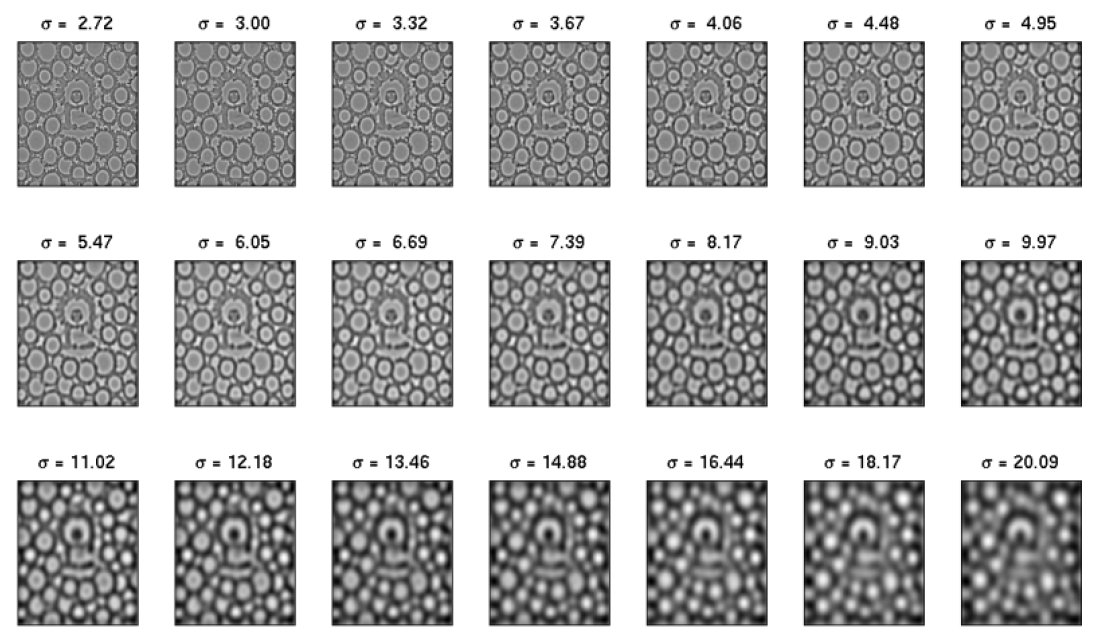
\includegraphics[width=\textwidth]{images/chap5/LOG_norm}

\begin{itemize}
    \item Factor $\sigma^2$ req. for true \textbf{scale invariance}
    \item Structures appear and vanish (bandpass behavior)
    \item At \textbf{characteristic scale} of feature, magnitude of NLoG takes extrema (min. or max.)
    \item Computing extrema in scale and space provides \textbf{location} and \textbf{scale} of features
    \item Simple case: extrema of NLoG can be found by comparing with direct neighbors in scale and space (doesn't have to be this way!)
\end{itemize}

\subsection{Step 2: Accurate Localisation of Key Points}

\textbf{Step 2a: Sub-pixel refinement}

Determine sub-pixel location of extemas by performing second order Taylor Expansion (poly. fit) around each feature point $\mathbf{x_i} = (x_i, y_i, \sigma_i)$ for distance $\mathbf{h}$:

$$D(\mathbf{x_i} + \mathbf{h}) \approx D(\mathbf{x_i}) + \nabla D(\mathbf{x_i})^T \mathbf{h} + \frac{1}{2} \mathbf{h}^T H(x_i) \mathbf{h}$$

$\nabla D$ being the gradient, $H = H(D)$ the hessian of the scale-space function, which can be approx. locally by central differences using neighbor pixels.

\textbf{Hessian:} $3\times 3$ symmetric matrix of mixed second derivative (is a tensor), the \textbf{gradient} a $3\times 1$ column vector.

\textbf{Condition} for extrema locations is given by setting the \textbf{derivative of quadratic approx. to zero}: $ \nabla D(\mathbf{x_i}) + H(\mathbf{x_i}) \mathbf{h} = 0$. Offset to extremum is given b $\hat{\mathbf{h}} = - H(\mathbf{x_i})^{-1} \nabla D(\mathbf{x_i})$. \textbf{New location} is $\hat{\mathbf{x_i}} = \mathbf{x_i + \hat{h}}$. Replacing $\mathbf{h, \hat{h}}$ in the function yields

$$D(\mathbf{\hat{x}_i}) = D(\mathbf{x_i}) + \frac{1}{2} \nabla D(\mathbf{x_i})^T \mathbf{\hat{h}}$$

\textbf{Improves accuracy of feature locations w.r.t. scale and location!}

\textbf{Step 2b: Elimate weak detections}

Discard iff $D(\mathbf{\hat{x}_i})$ is below threshold (paper use 0.03). Eliminates unreliable features in regions with low contrast.

\textbf{Step 2c: Elimination of unstable features}

Based on \textbf{principal curvatures:} Measures how surface bends in different directions. \textbf{Goal:} Smallest ad largest bending have same sign and magnitude, then extremum is stable.

Eigenvalues $\lambda_1 \geq \lambda_2$ of spatial Hessian $H_2 = \left[ \begin{matrix}
D_{xx} & D_{xy} \\
D_{yx} & D_{yy}
\end{matrix}\right]$

proportional to principal curvatures at $x,y$. For small ratios $r = \lambda_1 / \lambda_2 \geq 1$, the following expr. is minimized (does not need eigenvalue computation directly): $$\mathcal{K} = \dfrac{trace(H_2)^2}{det(H_2)} = \dfrac{(\lambda_1 + \lambda_2)^2}{\lambda_1\lambda_2} = \dfrac{(r+1)^2}{r} = r + 2 + \frac{1}{r}$$.

Discarding features iff, $det(H_2) < 0$, "saddle points" instead of extrema, $det(H_2) = 0$ no extrema. $\mathcal{K} > 10$, looks like ridge/valley instead of peak!

\subsection{Step 3: Assignment of dominant orientations}

\textbf{HoG:} For each feature point $\mathbf{x_i}$. Computed from gradients for $\hat{\sigma}_i$. Histogram using 36 bins (360°), weighted by magnitude of gradient and with gaussian centered at $(\hat{x}_i, \hat{y}_i)$, with STD $1.5\hat{\sigma}_i$.

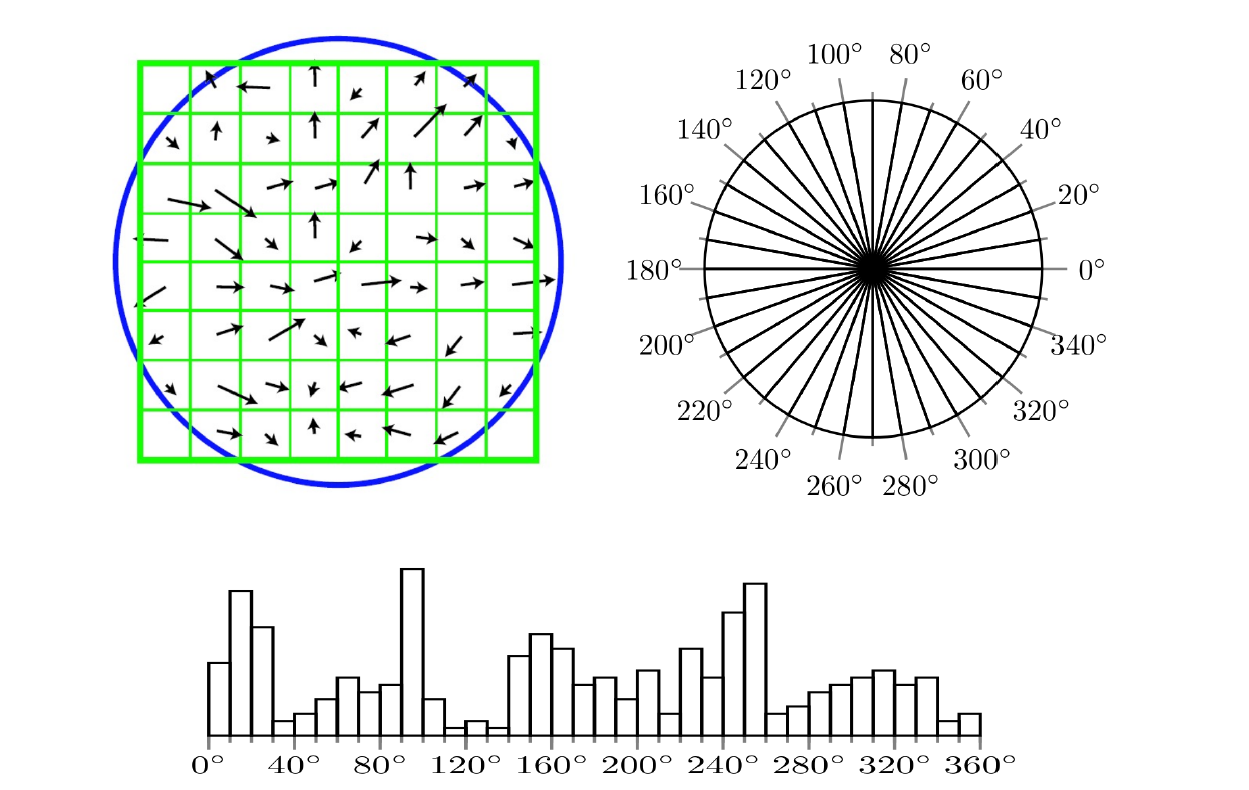
\includegraphics[width=\textwidth]{images/chap5/HoG}

Arrows: Gradients in circular neighborhood. \textbf{Blue} circle, $3\sigma$ of gaussian use for weighting. Histogram is created by angles. \textbf{Dominant} orientation is given by largest entry!

\textbf{Feature cloning for multiple dominant orientations:} Separate feature point for every entry that is above $80\%$ of value of dominant orientation. Sub-bin refinement is applied as well (1D).

Assignment looks like

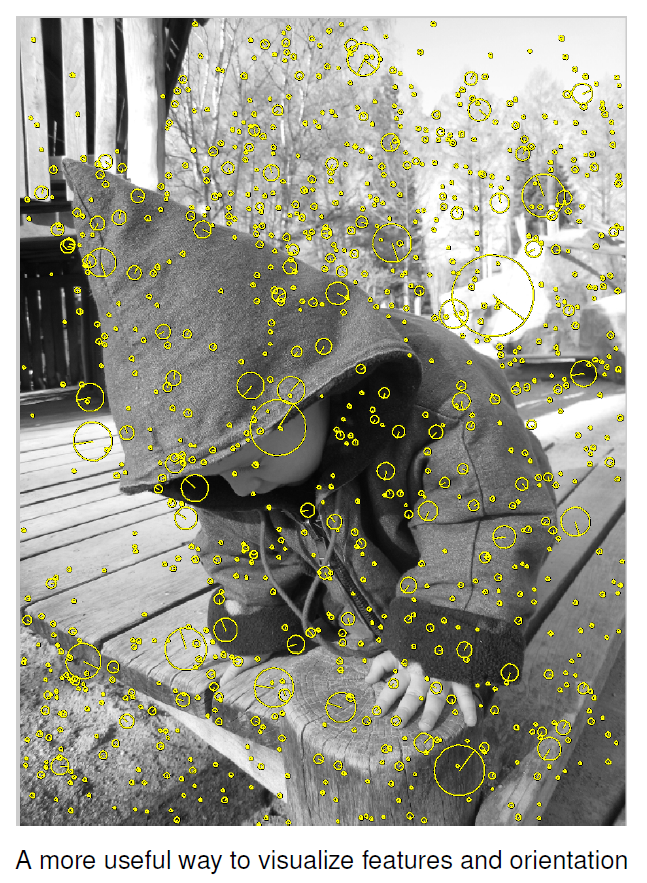
\includegraphics[width=.4\textwidth]{images/chap5/ori_asg}

\textbf{Step 4: Computation of suitable key point descriptors}

\textbf{Goal:} Unique representation of feature points by characteristic vectors.

\textbf{Block of HoGs:} Same as in orientation assignment (consider scale and location, mag. weighting, gaussian weighting). \textbf{Additionally}, sample location and gradient directions and rotate patch into "default" direction. Neighborhood divided in 16 blocks of $4\times 4$. Histograms using 8 bins, covering $45°$.

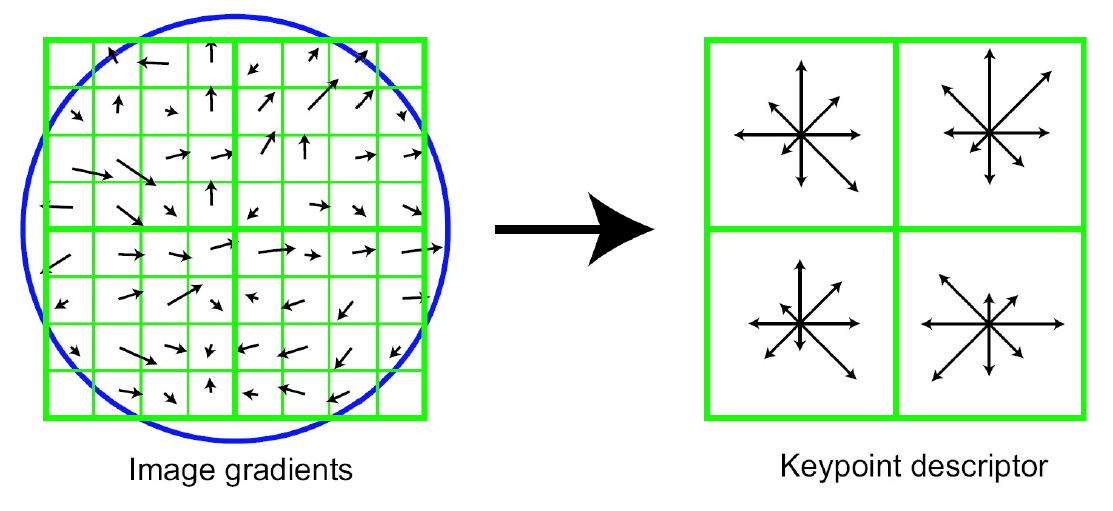
\includegraphics[width=.6\textwidth]{images/chap5/block_hog}

Example 4 blocks of $4\times 4$, i.e., 64 features. SIFT uses 16 blocks!. Right pictures is the keypoint descriptor as \textbf{HoG}.

\textbf{Problems:} Slight rotations/translations contribute same gradients to different bins (possibly).

\textbf{Solution:} Dist. votes of each gradient to neighboring bins and four neighboring blocks based on angular and spatial distance.

\section{SIFT Descriptor}

Stored for every feature, size 128 with 8 entries for 16 block histograms, for matching FD are compared computing euclidean norm of differences.

\textbf{Successful SIFT:}

\begin{itemize}
    \item Invariance under scaling, shift and rotation (information computed at characteristic scale by dominant orientation)
    \item Invariance under affine illumination changes (gradient is invariant for additive illumination, normailzation makes it invariant for multiplicative illumination changes)
    \item up to 60 degrees out of plane rotation demonstrated to still work quite well!
\end{itemize}

















